\section{Cơ Sở Lý Thuyết }

% 2.1
\subsection{Khái niệm kiến trúc đa nền tảng}
\renewcommand{\labelitemi}{--}

\subsubsection{Định nghĩa}
\begin{flushleft}
    \hspace*{0.8cm}Kiến trúc đa nền tảng (cross-platform architecture) là một phương pháp phát triển ứng dụng dựa trên một bộ mã nguồn chung, giúp triển khai đồng thời trên nhiều hệ điều hành như iOS, Android, cũng như các nền tảng khác như web hoặc desktop. Thay vì xây dựng từng phiên bản riêng biệt cho từng hệ điều hành, lập trình viên sử dụng các framework hoặc công cụ trung gian để biên dịch mã nguồn và tối ưu hóa cho từng môi trường cụ thể.
\end{flushleft}

\begin{flushleft}
    \hspace*{0.8cm}Các framework tiêu biểu cho kiến trúc đa nền tảng bao gồm:
    \setlength{\leftmargini}{1.5cm}
    \begin{itemize}
        \item \textbf{React Native}: Sử dụng JavaScript và biên dịch mã qua "bridge" thành mã máy tương ứng (Objective-C/Swift cho iOS, Java/Kotlin cho Android).
        \item \textbf{Flutter}: Dựa trên ngôn ngữ Dart và sử dụng Skia Engine để render giao diện trực tiếp, độc lập với hệ điều hành.
    \end{itemize}
\end{flushleft}

\subsubsection{Nguyên tắc "Write Once, Run Anywhere" (WORA)}
\begin{flushleft}
    \hspace*{0.8cm}Nguyên tắc WORA, được Sun Microsystems giới thiệu từ thập niên 1990, nhấn mạnh vào khả năng tái sử dụng mã nguồn tối đa và giảm chi phí phát triển. Nguyên tắc này dựa trên hai yếu tố cốt lõi:
    \setlength{\leftmargini}{1.5cm}
    \begin{itemize}
        \item \textbf{Tính độc lập nền tảng}: Mã nguồn không bị phụ thuộc vào hệ điều hành hoặc phần cứng cụ thể.
        \item \textbf{Tính nhất quán}: Logic nghiệp vụ và giao diện hoạt động đồng bộ trên mọi thiết bị.
    \end{itemize}
\end{flushleft}

\begin{flushleft}
    \hspace*{0.8cm}Một số ứng dụng thực tế đã áp dụng hiệu quả nguyên tắc này:
    \setlength{\leftmargini}{1.5cm}
    \begin{itemize}
        \item \textbf{Microsoft Teams}: Dùng React Native để triển khai trên iOS, Android và Windows với hơn 90\% mã nguồn dùng chung.
        \item \textbf{Google Pay}: Xây dựng trên Flutter, hỗ trợ cả mobile và web từ một codebase duy nhất.
    \end{itemize}
\end{flushleft}

\subsubsection{Lợi ích của kiến trúc đa nền tảng}
\begin{flushleft}
    \hspace*{0.8cm}So với phát triển native, kiến trúc đa nền tảng mang lại nhiều lợi ích về mặt chi phí, thời gian và khả năng bảo trì:
    \setlength{\leftmargini}{1.5cm}
    \begin{itemize}
        \item \textbf{Tiết kiệm thời gian và chi phí}: Theo InfoQ (2022), thời gian phát triển có thể giảm 50–80\%, đồng thời chỉ cần một đội ngũ phát triển thay vì nhiều nhóm chuyên biệt.
        \item \textbf{Ví dụ thực tế}: Startup DeliveryNow tiết kiệm được 300,000 USD trong vòng 12 tháng khi sử dụng Flutter cho cả iOS và Android.
        \item \textbf{Bảo trì dễ dàng}: Việc cập nhật tính năng hoặc sửa lỗi được thực hiện một lần và áp dụng đồng thời cho mọi nền tảng.
        \item \textbf{Tích hợp CI/CD}: Quy trình phát hành được tự động hóa, giảm rủi ro và nâng cao tốc độ triển khai.
    \end{itemize}
\end{flushleft}

\subsubsection{Thách thức và hạn chế}
\begin{flushleft}
    \hspace*{0.8cm}Mặc dù mang lại nhiều lợi thế, kiến trúc đa nền tảng vẫn tồn tại những điểm hạn chế nhất định:
    \setlength{\leftmargini}{1.5cm}
    \begin{itemize}
        \item \textbf{Hiệu năng thấp hơn native}: Theo Biorn-Hansen (2021), ứng dụng đa nền tảng có thể chậm hơn 15–30\% khi xử lý đồ họa nặng như animation hoặc game 3D.
        \item \textbf{Ví dụ}: Pokémon GO từng thử nghiệm với Unity (cross-platform) nhưng phải chuyển sang native do hiện tượng lag khi render bản đồ 3D.
        \item \textbf{Khó tùy chỉnh giao diện}: Các framework đa nền tảng sử dụng UI tổng quát, khó đáp ứng đặc trưng thiết kế như Material Design (Android) hay Cupertino (iOS).
        \item \textbf{Ví dụ}: Spotify (React Native) phải viết lại nhiều thành phần UI bằng mã native để đảm bảo trải nghiệm người dùng.
        \item \textbf{Phụ thuộc vào cộng đồng và công cụ}: Nhiều plugin do cộng đồng phát triển có thể thiếu ổn định hoặc ngừng duy trì.
        \item \textbf{Ví dụ}: React Native Maps từng gặp lỗi nghiêm trọng trên iOS 14, dẫn đến crash hàng loạt.
    \end{itemize}
\end{flushleft}

\subsubsection{Công cụ phát triển}
\begin{flushleft}
  \hspace*{0.8cm}Phát triển ứng dụng đa nền tảng đòi hỏi lập trình viên sử dụng các công cụ chuyên biệt nhằm tối ưu quy trình xây dựng, kiểm thử và triển khai. Những công cụ này bao gồm IDE (môi trường phát triển tích hợp), bộ giả lập thiết bị, công cụ kiểm thử và hệ thống quản lý mã nguồn.

  \begin{figure}[H]
    \centering
    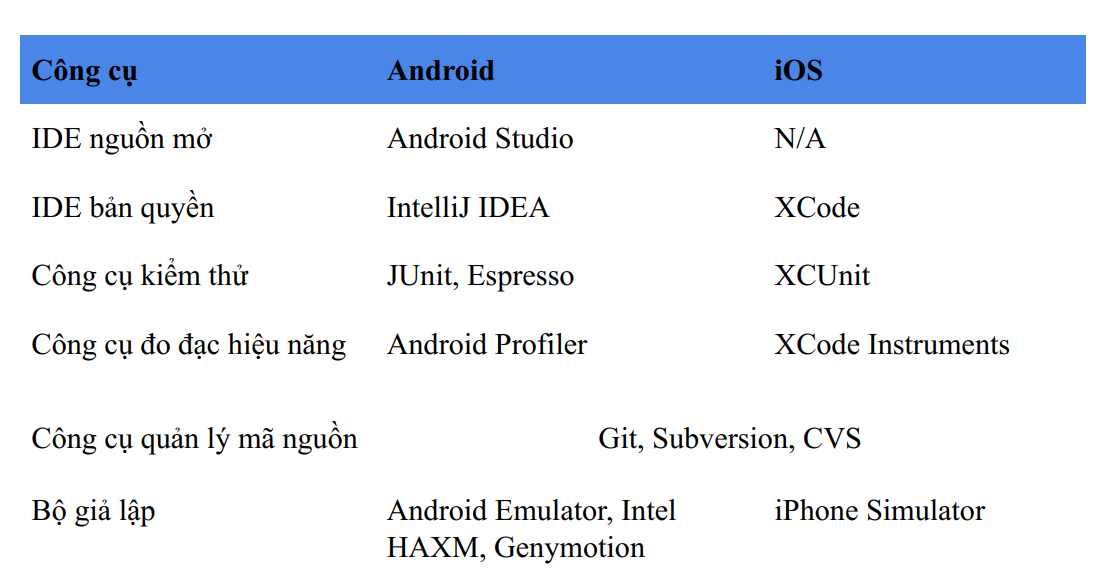
\includegraphics[width=0.95\textwidth]{images/cong-cu-android-ios.png}
    \caption{So sánh công cụ phát triển giữa Android và iOS}
    \label{fig:android_ios_tools}
  \end{figure}

  \hspace*{0.8cm}Hình~\ref{fig:android_ios_tools} thể hiện sự khác biệt giữa các công cụ được sử dụng trong hệ sinh thái Android và iOS. Việc lựa chọn công cụ phù hợp phụ thuộc vào hệ điều hành mục tiêu, ngôn ngữ lập trình và kinh nghiệm của lập trình viên.
\end{flushleft}


% 2.2
\subsection{Các yếu tố quyết định khi lựa chọn đa nền tảng}
\renewcommand{\labelitemi}{--}    
\begin{flushleft}

  \subsubsection{Phân tích nhóm người dùng mục tiêu}
    \begin{flushleft}
      \hspace*{0.8cm}Thị phần hệ điều hành đóng vai trò quan trọng trong việc xác định nền tảng ưu tiên.
      \setlength{\leftmargini}{1.5cm}
      \begin{itemize}
        \item iOS hiện chiếm 27\% thị trường toàn cầu, chủ yếu phổ biến tại Mỹ và Châu Âu.
        \item Android chiếm 73\%, đặc biệt thống trị tại Châu Á và Châu Phi (Statista, 2023).
      \end{itemize}
    \end{flushleft}

    \begin{flushleft}
      \hspace*{0.8cm}Chiến lược tiếp cận người dùng cần phù hợp với đặc thù từng hệ điều hành.
      \setlength{\leftmargini}{1.5cm}
      \begin{itemize}
          \item Nếu đối tượng mục tiêu là người dùng cao cấp (iOS), nên ưu tiên framework hỗ trợ giao diện Cupertino như Flutter.
          \item Nếu nhắm tới thị trường đại chúng (Android), React Native là lựa chọn phù hợp nhờ khả năng tích hợp với Google Services.
      \end{itemize}
    \end{flushleft}

    \begin{flushleft}
      \hspace*{0.8cm}Một ví dụ thực tế giúp minh họa rõ ràng cho lựa chọn nền tảng là Grab.
      \setlength{\leftmargini}{1.5cm}
      \begin{itemize}
          \item Grab (Flutter): Tập trung vào thị trường Đông Nam Á (đa số dùng Android) nhưng vẫn đảm bảo trải nghiệm mượt mà trên iOS.
      \end{itemize}
    \end{flushleft}

    \subsubsection{Mô hình "Rẻ – Nhanh – Tốt"}
    \begin{flushleft}
      \hspace*{0.8cm}Nguyên tắc Iron Triangle cho rằng chỉ có thể đạt hai trong ba tiêu chí: rẻ, nhanh và tốt. Mỗi lựa chọn framework cần cân nhắc dựa trên ưu tiên này.
    \end{flushleft}
    
    \begin{flushleft}
      \centering
      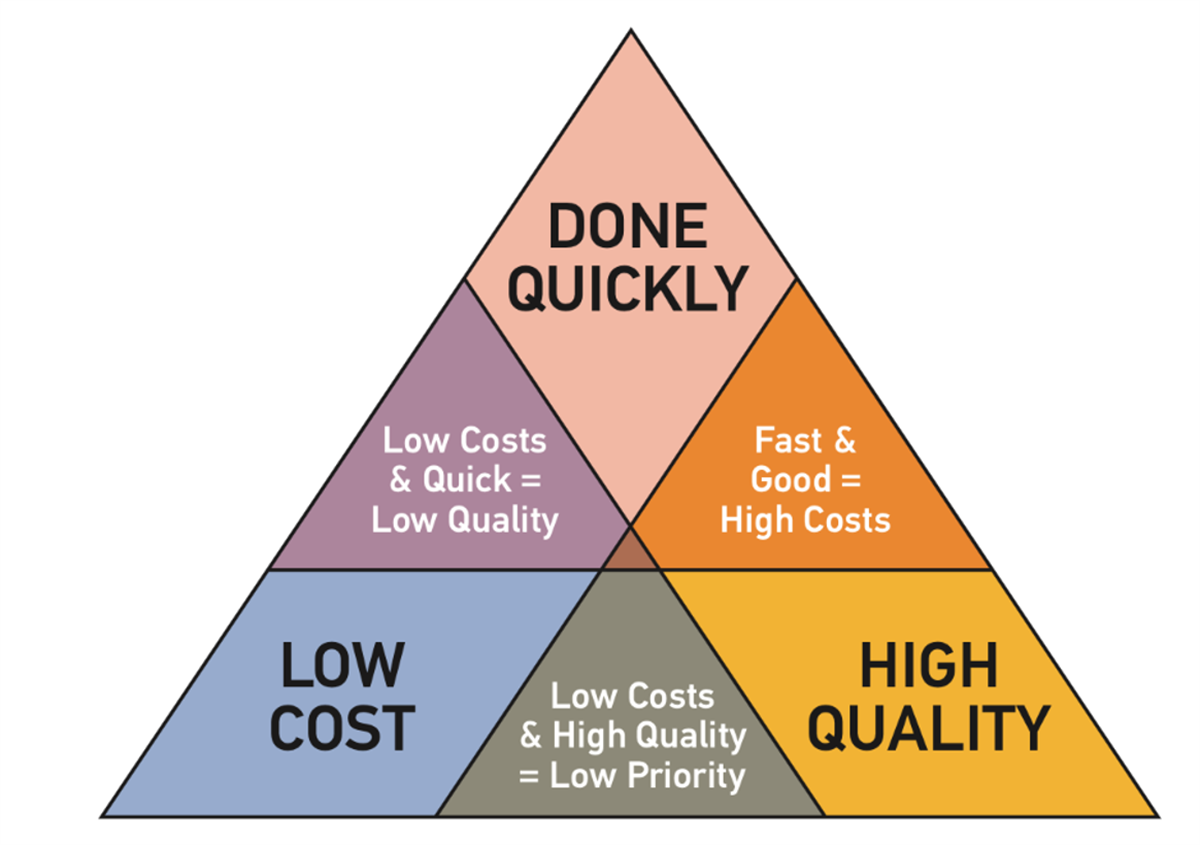
\includegraphics[width=0.45\textwidth]{images/iron_triangle.png} \\
      \textit{\small Hình: Mô hình Iron Triangle – Rẻ, Nhanh, Tốt – Chọn hai}
    \end{flushleft}
    
    \begin{flushleft}
      \hspace*{0.8cm}Tùy vào mục tiêu dự án, mỗi framework sẽ phù hợp với một chiến lược khác nhau.
      \setlength{\leftmargini}{1.5cm}
      \begin{itemize}
          \item React Native: Phù hợp cho dự án cần MVP (Minimum Viable Product) nhanh chóng, nhưng hiệu năng không cao.
          \item Flutter: Đòi hỏi đầu tư ban đầu để học Dart, nhưng mang lại hiệu năng cao và giao diện tùy biến tốt hơn.
      \end{itemize}
    \end{flushleft}
    

  \subsubsection{Khả năng tích hợp với hệ sinh thái hiện có}
    \begin{flushleft}
      \hspace*{0.8cm}React Native tận dụng tốt hệ sinh thái JavaScript (Node.js, npm, Expo) và dễ tích hợp với ứng dụng web hiện tại.
    \end{flushleft}

    \begin{flushleft}
      \hspace*{0.8cm}Flutter mặc dù độc lập hơn, nhưng vẫn có thể kết nối hiệu quả với Firebase hoặc Google Cloud thông qua plugin.
    \end{flushleft}

    \begin{flushleft}
      \hspace*{0.8cm}Một ví dụ điển hình cho khả năng tích hợp là Shopify.
      \setlength{\leftmargini}{1.5cm}
      \begin{itemize}
          \item Shopify sử dụng React Native để tích hợp ứng dụng mobile với nền tảng web sẵn có.
      \end{itemize}
    \end{flushleft}

\end{flushleft}


% 2.3
\subsection{Lịch sử phát triển của kiến trúc đa nền tảng}
\renewcommand{\labelitemi}{--}    
\begin{flushleft}

  \subsubsection{Thế hệ đầu tiên (2010–2015): WebView-based Frameworks}
  
  \begin{flushleft}
    Giai đoạn đầu tiên trong kiến trúc đa nền tảng là sự xuất hiện của các framework dựa trên WebView. 
    \textbf{Công cụ tiêu biểu} gồm: PhoneGap, Cordova, và Ionic.
  \end{flushleft}

  \begin{flushleft}
    Các framework này hoạt động bằng cách đóng gói nội dung HTML/CSS/JavaScript trong WebView, 
    tức là bản chất ứng dụng chỉ là một trình duyệt bên trong native shell.
  \end{flushleft}

  \begin{flushleft}
    \textbf{Ưu điểm} của cách tiếp cận này là:
    \setlength{\leftmargini}{1.5cm}
    \begin{itemize}
      \item Lập trình viên web có thể dễ dàng tiếp cận và phát triển ứng dụng.
      \item Chi phí phát triển và bảo trì thấp.
    \end{itemize}
  \end{flushleft}

  \begin{flushleft}
    Tuy nhiên, \textbf{hạn chế} rõ ràng nhất là:
    \setlength{\leftmargini}{1.5cm}
    \begin{itemize}
      \item Hiệu năng thấp, không xử lý tốt các animation phức tạp.
      \item Giao diện không mượt, thiếu tính bản địa hoá do không sử dụng native UI components.
    \end{itemize}
  \end{flushleft}

  \begin{flushleft}
    Một ví dụ điển hình là ứng dụng Uber: 
    ban đầu phát triển bằng Cordova nhưng phải chuyển sang native do hiện tượng lag khi hiển thị bản đồ.
  \end{flushleft}

  \vspace{0.5cm}
  \subsubsection{Thế hệ thứ hai (2015–2017): Hybrid Frameworks}
  
  \begin{flushleft}
    Sau WebView, thế hệ thứ hai đã ra đời với nỗ lực kết hợp WebView và native components, 
    gọi là Hybrid Frameworks. \textbf{Các công cụ tiêu biểu} là Xamarin và NativeScript.
  \end{flushleft}

  \begin{flushleft}
    Cơ chế hoạt động của chúng dựa vào \textit{bridge} để kết nối code JavaScript (hoặc C\#) với native APIs, cho phép sử dụng một số thành phần giao diện bản địa.
    \end{flushleft}

  \begin{flushleft}
    \textbf{Ưu điểm} nổi bật:
    \setlength{\leftmargini}{1.5cm}
    \begin{itemize}
      \item Hiệu năng được cải thiện đáng kể so với thế hệ WebView.
      \item Truy cập được các native APIs như camera, GPS.
    \end{itemize}
  \end{flushleft}

  \begin{flushleft}
    Tuy vậy, vẫn còn \textbf{nhiều hạn chế}:
    \setlength{\leftmargini}{1.5cm}
    \begin{itemize}
      \item Quá trình cấu hình phức tạp và dễ lỗi.
      \item Một số phần vẫn phụ thuộc vào WebView.
    \end{itemize}
  \end{flushleft}

  \begin{flushleft}
    Ví dụ điển hình: Microsoft Outlook ứng dụng Xamarin để phát triển ứng dụng đa nền tảng một cách hiệu quả.
  \end{flushleft}

  \vspace{0.5cm}
  \subsubsection{Thế hệ hiện đại (2017–nay): Native-Reactive Frameworks}
  
  \begin{flushleft}
    Từ năm 2017 đến nay, kiến trúc đa nền tảng bước sang giai đoạn hiện đại với sự xuất hiện của 
    các \textbf{framework reactive sử dụng native rendering}. Tiêu biểu là React Native và Flutter.
  \end{flushleft}

  \begin{flushleft}
    \textbf{Cơ chế hoạt động} của mỗi framework:
    \setlength{\leftmargini}{1.5cm}
    \begin{itemize}
      \item React Native: Dùng JavaScript để điều khiển native components thông qua bridge.
      \item Flutter: Dùng Dart và engine Skia để tự vẽ giao diện mà không phụ thuộc hệ điều hành.
    \end{itemize}
  \end{flushleft}

  \begin{flushleft}
    Nhờ cơ chế hiện đại, các framework này mang lại \textbf{nhiều ưu điểm}:
    \setlength{\leftmargini}{1.5cm}
    \begin{itemize}
      \item Hiệu năng gần tương đương ứng dụng native.
      \item Hỗ trợ đa nền tảng: từ mobile đến web và desktop.
    \end{itemize}
  \end{flushleft}

  \begin{flushleft}
    Một số \textbf{bước đột phá} quan trọng trong giai đoạn này:
    \setlength{\leftmargini}{1.5cm}
    \begin{itemize}
      \item Flutter 2.0 (2020): Mở rộng hỗ trợ cho nền tảng web và desktop.
      \item React Native New Architecture (2022): Ứng dụng TurboModules và Fabric để tối ưu hiệu suất.
    \end{itemize}
  \end{flushleft}

  \begin{flushleft}
    Một ví dụ thành công: Ứng dụng Xianyu của Alibaba sử dụng Flutter để phục vụ hơn 200 triệu người dùng, 
    đạt hiệu năng tương đương ứng dụng native.
  \end{flushleft}
\end{flushleft}
% 2.4
\subsection{Xu hướng tương lai của kiến trúc đa nền tảng}
\renewcommand{\labelitemi}{--}

\subsubsection{Tích hợp AI/ML trong phát triển}

Một trong những xu hướng quan trọng là việc tích hợp trí tuệ nhân tạo và học máy vào quy trình phát triển ứng dụng đa nền tảng.  
Thông qua công cụ như Google’s ML Kit, lập trình viên có thể tự động hóa các tác vụ như nhận diện hình ảnh và xử lý ngôn ngữ tự nhiên.

AI không chỉ hỗ trợ tính năng thông minh, mà còn giúp tối ưu hiệu năng ứng dụng.  
Cụ thể, các hệ thống AI có thể phân tích mã nguồn để đề xuất cải thiện tốc độ khung hình (FPS) hoặc giảm tiêu thụ bộ nhớ RAM.

Một ví dụ điển hình là Adobe XD, trong đó AI được sử dụng để tự động điều chỉnh giao diện người dùng dựa trên hành vi thực tế của người dùng.

\vspace{0.5cm}

\subsubsection{WebAssembly (Wasm) và Progressive Web Apps (PWA)}

WebAssembly đang nổi lên như một công nghệ quan trọng giúp ứng dụng chạy trên trình duyệt với hiệu năng gần tương đương ứng dụng native.  
Khả năng này giúp mở rộng phạm vi triển khai ứng dụng đa nền tảng trên môi trường web một cách hiệu quả.

Cùng với đó, Progressive Web Apps (PWA) mang lại sự kết hợp giữa ứng dụng web và mobile app,  
hỗ trợ hoạt động offline và cho phép gửi thông báo đẩy đến người dùng như các ứng dụng native.

Một ví dụ tiêu biểu là Starbucks, hãng đã triển khai PWA để tăng tốc độ tải trang và nâng cao trải nghiệm người dùng ngay cả khi không có kết nối mạng ổn định.

\vspace{0.5cm}

\subsubsection{Low-Code/No-Code Platforms}

Low-code và no-code platforms đang mở ra cơ hội mới cho cả những người không chuyên trong lĩnh vực lập trình.  
Với các nền tảng kéo–thả trực quan, người dùng có thể xây dựng ứng dụng đa nền tảng mà không cần viết bất kỳ dòng code nào.

Lợi ích lớn nhất của mô hình này là rút ngắn thời gian phát triển và giảm thiểu chi phí đào tạo kỹ thuật,  
đặc biệt phù hợp với doanh nghiệp nhỏ hoặc bộ phận nội bộ cần triển khai nhanh giải pháp công nghệ.

Chẳng hạn, Microsoft Power Apps đã giúp nhiều doanh nghiệp tạo ra ứng dụng quản lý nội bộ chỉ trong vài giờ làm việc.


% 2.5
\subsection{Case Study Chi Tiết}
\renewcommand{\labelitemi}{--}

\subsubsection{Airbnb và bài học từ React Native}

Airbnb đã từng áp dụng React Native với kỳ vọng tận dụng khả năng chia sẻ code giữa các nền tảng.  
Tuy nhiên, trong quá trình phát triển, họ gặp phải một số thách thức lớn.

Cụ thể, nhóm phát triển gặp khó khăn trong việc tùy chỉnh giao diện người dùng phức tạp cho từng nền tảng,  
đặc biệt là khi phải đảm bảo trải nghiệm nhất quán và mượt mà.

Ngoài ra, hiệu năng ứng dụng không đủ đáp ứng yêu cầu khi tích hợp tính năng đặt phòng theo thời gian thực,  
gây ảnh hưởng đến trải nghiệm người dùng cuối.

Để giải quyết vấn đề này, Airbnb quyết định chuyển sang phát triển native cho các module quan trọng,  
đồng thời giữ lại React Native cho phần quản trị nội bộ nhằm tiết kiệm chi phí.

Kết quả của chiến lược này là hiệu năng hệ thống được cải thiện 30\%,  
nhưng chi phí bảo trì cũng tăng lên khoảng 40\% do cần duy trì song song hai mã nguồn.

\vspace{0.5cm}

\subsubsection{Google Pay: Thành công với Flutter}

Google Pay là một trong những ví dụ điển hình cho việc ứng dụng thành công Flutter vào phát triển đa nền tảng.  
Chiến lược của nhóm phát triển là sử dụng một codebase duy nhất cho cả iOS, Android và web.

Nhờ khả năng đồng bộ cao của Flutter, thời gian phát triển đã giảm tới 50\%,  
giúp nhóm ra mắt sản phẩm nhanh hơn mà vẫn đảm bảo chất lượng.

Bên cạnh đó, hiệu năng ứng dụng cũng được đảm bảo, với tốc độ khung hình (FPS) ổn định ở mức 60 trên mọi thiết bị,  
tạo nên trải nghiệm người dùng mượt mà và đáng tin cậy.

Tuy nhiên, nhóm cũng đối mặt với thách thức trong việc đào tạo đội ngũ kỹ thuật,  
đặc biệt là làm quen với ngôn ngữ Dart và cơ chế vẽ giao diện qua Skia Engine.

% 2.6
\subsection{So Sánh Chi Tiết React Native vs. Flutter}
\renewcommand{\labelitemi}{--}    
\begin{flushleft}
    \hspace*{0.8cm}Biểu đồ dưới đây so sánh mức độ quan tâm giữa hai framework di động phổ biến: \textbf{Flutter (xanh)} và \textbf{React Native (đỏ)} trong 12 tháng qua tại Hoa Kỳ, dựa trên dữ liệu tìm kiếm từ Google Trends.

    \begin{figure}[H]
        \centering
        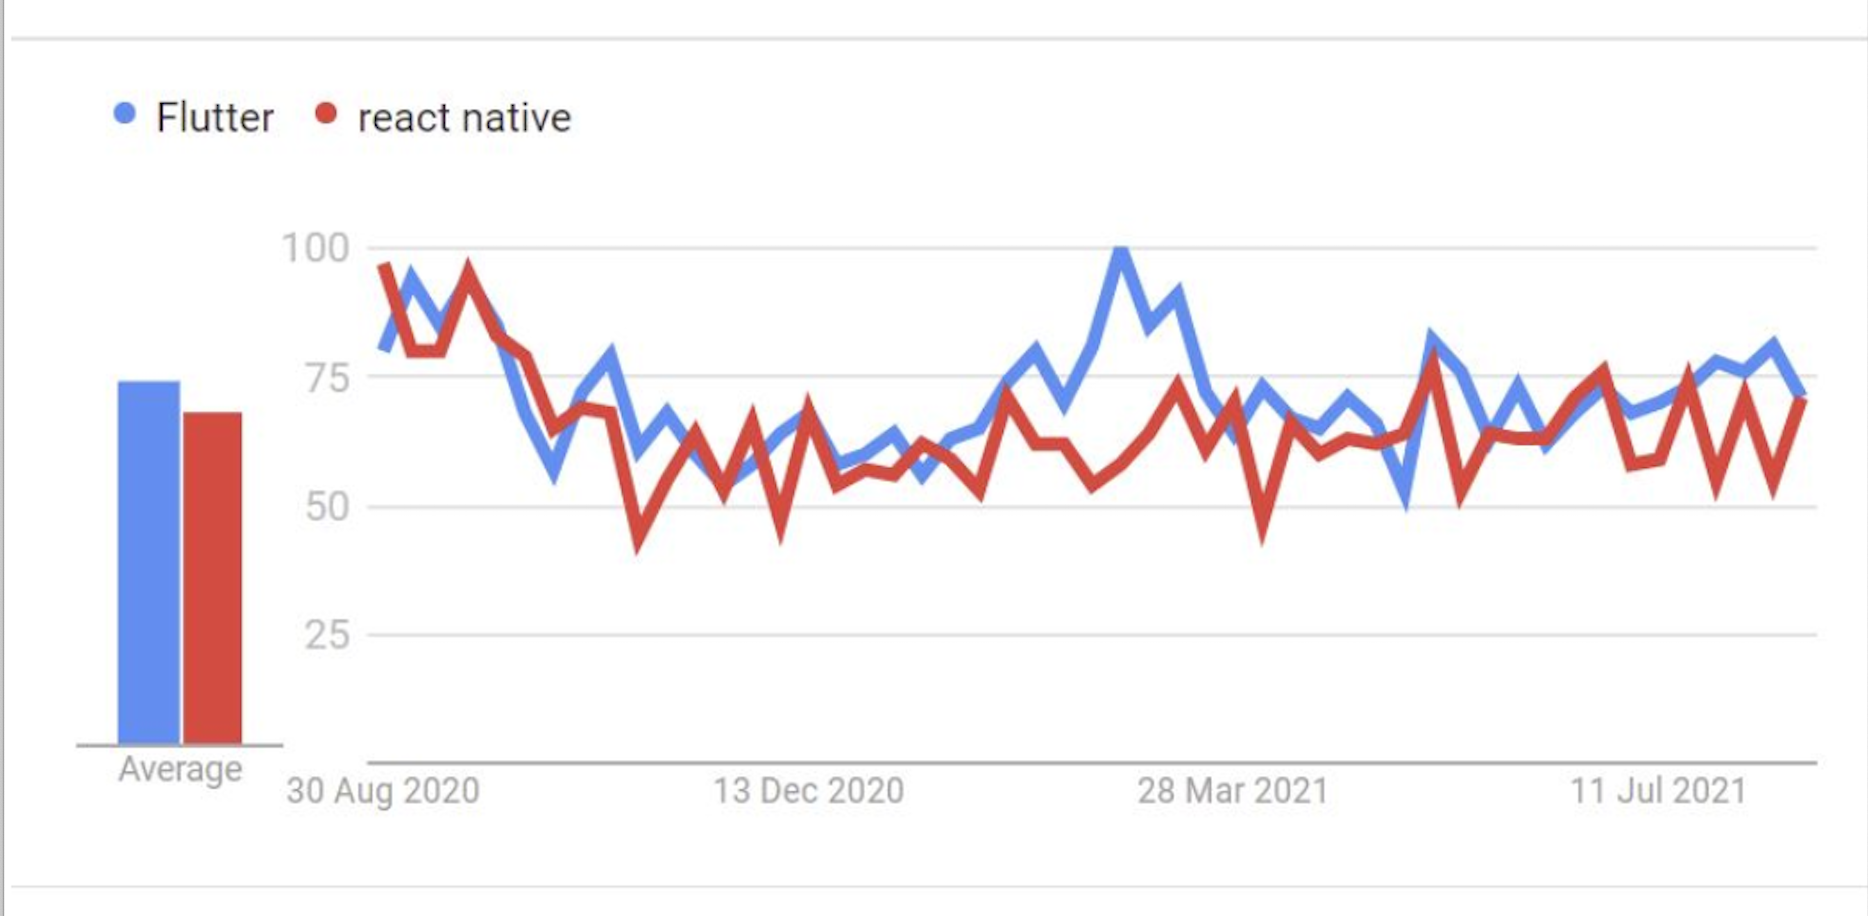
\includegraphics[width=0.9\textwidth]{images/reactNative_flutter.png}
        \caption{So sánh xu hướng tìm kiếm giữa Flutter và React Native (Google Trends, US, 12 tháng)}
    \end{figure}

    \vspace{0.5cm}
    Dưới đây là bảng so sánh một số khía cạnh chính giữa React Native và Flutter:

    \begin{table}[H]
        \centering
        \begin{tabular}{|l|p{6cm}|p{6cm}|}
            \hline
            \textbf{Tiêu chí} & \textbf{React Native} & \textbf{Flutter} \\
            \hline
            Ngôn ngữ lập trình & JavaScript (hoặc TypeScript) & Dart \\
            \hline
            Hiệu suất & Gần với native, phụ thuộc vào bridge & Cao hơn nhờ rendering engine riêng (Skia) \\
            \hline
            Giao diện người dùng & Dựa vào native components & Tùy chỉnh hoàn toàn, nhất quán mọi nền tảng \\
            \hline
            Cộng đồng & Lâu đời hơn, cộng đồng lớn & Đang phát triển nhanh chóng, được Google hỗ trợ mạnh \\
            \hline
            Tài liệu & Đầy đủ, nhiều ví dụ thực tiễn & Rõ ràng, cấu trúc tốt, phù hợp cho người mới bắt đầu \\
            \hline
        \end{tabular}
        \caption{So sánh các yếu tố giữa React Native và Flutter}
    \end{table}
\end{flushleft}

% 2.7
\subsection{Kết luận phần Cơ Sở Lý Thuyết}
\renewcommand{\labelitemi}{--}    
    \begin{flushleft}
        \hspace*{0.8cm}Kiến trúc đa nền tảng đã phát triển qua nhiều giai đoạn, từ các giải pháp dựa trên WebView đến các framework hiện đại như React Native và Flutter. Mỗi công cụ có ưu nhược điểm riêng, phù hợp với từng loại dự án. Việc lựa chọn phụ thuộc vào sự cân nhắc giữa chi phí, thời gian, và chất lượng, cùng với định hướng dài hạn của doanh nghiệp. Xu hướng tương lai hứa hẹn sự tích hợp sâu rộng của AI, WebAssembly và low-code platforms, mở ra kỷ nguyên mới cho phát triển ứng dụng linh hoạt và hiệu quả.
    \end{flushleft}